\section{Technical Stack}
\subsection{Technologies Used}
For what platform to distribute our solution on, it was felt that a mobile solution was the most applicable. Ideally apps exist on both the Google Play Store as well as the Apple App Store, however due to time constraints, we chose to stick to one platform, that being the latter iOS. A large factor for this decision was because members of the group have experience developing iOS applications, and hence this would ultimately speed up development. For a similar reason, Objective-C was chosen for development. However, for future versions, developers may decide to switch over to Swift, as there certainly are benefits to this language, but it did not make sense for us at the time.
\subsection{Implementation}
\subsubsection{User Interface Design Process}
The first step after identifying iOS as the most suitable platform, is to convert the product requirements to user experience flows. From there the design process begins with the following steps:
\begin{enumerate}
    \item Ideation
    \item Sketches
    \item Lo-fi mockups
    \item Design Reviews
\end{enumerate}
One aspect of design that was important to keep in mind was the Apple Human Interface Guidelines\footnote{\url{https://developer.apple.com/design/human-interface-guidelines/}}. Apple is quite strict on ensuring that apps on their plateform follow this guidelines. There are six main design principles that need to be followed: Aesthetic Integrity, Consistency, Direct Manipulation, Feedback, Metaphors and User Control.
\newline \newline
For building our user experience flows, it was chosen to use a combination of Xcode Storyboards and coupled with programming flows in code. In the future, moving to SwiftUI\footnote{\url{https://developer.apple.com/xcode/swiftui/}} would be beneficial.
\begin{figure}[h]
\centering
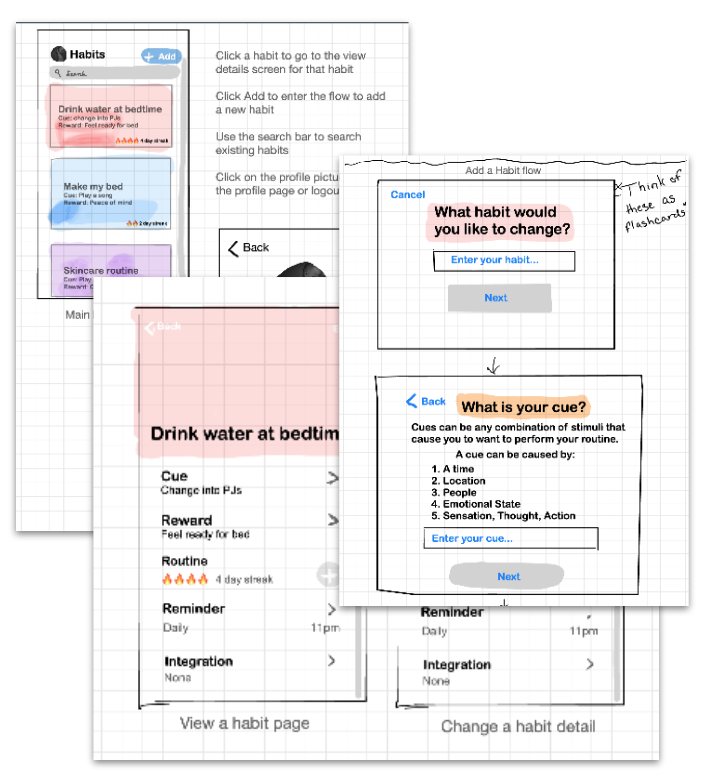
\includegraphics[width=0.7\textwidth]{images/mockups.png}
\caption{Early lo-fi mockups}
\end{figure}
\subsubsection{Backend and Database Services}
The current version of the iOS app utilizes Apple’s CoreData and CloudKit services, as opposed to a traditional backend. CoreData is a local store that effectively employs SQLite. While fairly light-weight, it has great development tools in Xcode for building database schemas and automatically generates the ORM models in your codebase. CoreData stores all the user information in the local storage of their iOS device, which is great from a security perspective. CloudKit on the other hand, is used to sync data between all of the devices associated with a user’s iCloud account. By using CloudKit habits added on one person’s iPhone, get pushed to their iPad, or even macOS devices (if there was a macOS app). Using both of these technologies was advantageous, as they were fairly easy to implement, and work consistently. The only disadvantage with its use is having to heavily lock your code into the Apple ecosystem. For a future iteration of this project, it may be worthwhile shifting to another dedicated backend solution, especially if there exists a desire to create an Android version alongside the iOS.
\begin{figure}[h]
\centering
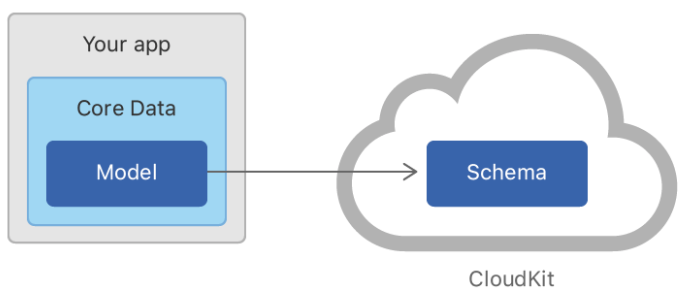
\includegraphics[width=0.55\textwidth]{images/cloudkit.png}
\caption{Basic CloudKit layout}
\end{figure}
\subsubsection{Security and Privacy}
\begin{itemize}
    \item \textbf{Sign in with Apple:} This feature allows users to have peace of mind about their privacy. ”Data collection is limited to the user’s name and email address, and Apple’s private email relay lets users receive email[s] even if they prefer to keep their address private. Apple will not track users as they interact with your app."\footnote{\url{https://developer.apple.com/sign-in-with-apple/}}. A benefit to using this feature, is that it moves the concern of data privacy from the application to Apple. Apple takes privacy very seriously to have their user’s data protected by their systems, as opposed to the applications taking on this responsibility, and is a great way to decrease the liability exposure of the application.
    \item \textbf{Habit Data:} As mentioned in section 4.2.2 the application utilizes the Apple CoreData and CloudKit for handling user data. While CoreData stores data locally on a user’s device, CloudKit uses iCloud syncing to transmit information, therefore, the potential for a user’s habit data to get compromised is very low. One easy solution is to allow users to toggle on and off CloudKit in their settings. Regardless of whether multi-device sync is enabled or not, the application backend is never able to see a user’s habit information that they enter, thereby removing another potential liability for the application.
\end{itemize}

\subsection{Potential Expansions}
If implementing these additions in future works, one must ensure that there is sufficient justification to do so. Adding features for ”the sake of adding features”, or ”because we need more technical complexity” are not valid justifications. Excessive bloat was found to be detrimental to many of the existing habit tracking apps on the various app stores. Herein, we discuss some ideas that were brought up during the development process but were never implemented.
\subsubsection{Health Data}
A lot of people try to make health-related habit improvements. For instance, drinking more water, exercising more, and eating less processed foods to name a few. In doing so, users can take advantage of health data that may be stored on their phone. Data from places such as the built-in pedometer and water tracker, and even third party apps such as MyFitnessPal, could be used. This could be extended to an Apple Watch compatible app as well, which would make this integration more accurate and powerful. For example the heart rate sensor in the watch can automatically detect periods of exercise, so in the case that one user’s habits involve ”going for a run during lunch break”, the watch could automatically detect and inform the app that the user has done their new routine.
\subsubsection{Financial Data}
Services like Plaid\footnote{\url{https://plaid.com/what-is-plaid/}}are easy for developers to use and allow users to integrate with over 11,000 different financial institutions. This could be used to help those who want to create financial-oriented habits like saving and investing money. In addition to Plaid, another app discovered called Alpaca \footnote{\url{https://alpaca.markets/}}, is an online only brokerage that has no market interface or GUI. You have to provide the full interface in Python yourself. It could be implemented to have users carry out automatic investing that apps like Acorns\footnote{\url{https://www.acorns.com/}} have been doing for years.
\subsubsection{Location Data}
Location data could be utilized by the app to assist in managing habits that involve a specific location as part of their cue. For instance, the app could send specific push notifications when users reach a certain geographical location, such as during reminding them to listen to an educational e-book during their commute, or buying healthy foods when they are in the proximity of the grocery store.

\subsubsection{Spotify API}
Spotify\footnote{\url{https://developer.spotify.com/documentation/web-api/}} has an API that can be used to play music clips within an application, as well as a variety of other features. This would not be investigated in much detail, but there was a motive that it may be useful for people that who have a music-based cue. Ultimately, the idea was dropped as it was too niche of a cue to focus on at such early developments of the app.
\subsubsection{IFTTT}
"IF This Then That"\footnote{\url{https://ifttt.com/}} is a service that can be used to register webhooks with actions in a wide variety of applications. It was not investigated in much detail, but it could potentially be later employed.